\section{Procedimentos}

\par Para que esta pesquisa fosse levada a cabo, se fez necessária a implementação de algumas ações, as quais serão detalhadas.

\par O início da pesquisa deu-se através da escolha do tema, seguido pelo levantamento das tecnologias que seriam utilizadas. A princípio, foi definido um escopo contendo algumas tecnologias que haviam sido ministradas no ambiente acadêmico, diminuindo assim a curva de aprendizado. No entanto, foi preciso agregar alguns conhecimentos novos, despendendo um tempo maior para estudo. As tecnologias empregadas no desenvolvimento deste trabalho foram: a linguagem de programação Java, o banco de dados orientado a grafos Neo4j, juntamente com a API Cypher, Tomcat, Primefaces e JSF, sendo que no decorrer do desenvolvimento prático, viu-se a necessidade de substituir as duas últimas tecnologias citadas pelas linguagens HTML, CSS, Javascript e pelo \textit{framework} Angular JS. As tecnologias que acompanharam o desenvolvimento deste trabalho até a sua conclusão estão descritas no quadro teórico desta pesquisa.

\par Para garantir que as tecnologias selecionadas fossem as melhores para o desenvolvimento, foram realizados alguns testes, por meio de aplicações simples. Os testes foram focados na avaliação do comportamento do banco de dados aplicado ao contexto desta pesquisa, cujo objetivo foi desenvolver uma aplicação de busca por mão de obra baseando-se em uma rede de relacionamentos. Estes testes também foram realizados como fins didáticos, visando gerar a familiarização com as tecnologias utilizadas.

\par Para nortear este trabalho, o ICONIX foi escolhido como a metodologia de desenvolvimento de \textit{software}, desempenhando um papel fundamental na organização. Sua abordagem proveu uma sequencia de procedimentos, que foram seguidos conforme o necessário, levando à construção de uma aplicação estável. Como relatado no quadro teórico, foram seguidas as quatro fases definidas pelo ICONIX.

\par Na primeira fase, definida como análise de requisitos, foi realizado o levantamento das informações pertinentes ao desenvolvimento. Este levantamento foi realizado por meio da observação do comportamento das pessoas ao buscar por mão de obra temporária. A partir dai, foram levantadas as principais características, indispensáveis para a construção do \textit{software} e desenvolvido o modelo de domínio inicial, como demonstra a Figura 15. Nesta fase, também foram definidas todas as ações que o usuário poderia realizar no sistema, por meio dos casos de uso, conforme a Figura 16.

\newpage
\begin{figure}[h!]
	\centerline{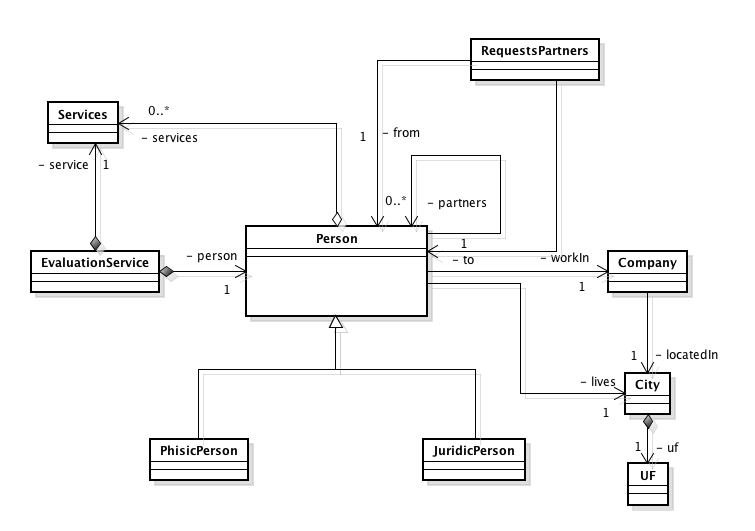
\includegraphics[scale=0.45]{./imagens/modelo-dominio-inicial.png}}
	\caption[Modelo de domínio inicial]
	{Modelo de domínio inicial. \textbf{Fonte:} Elaborado pelos autores.}
	\label{fig:exemplo1}
\end{figure}

\begin{figure}[h!]
	\centerline{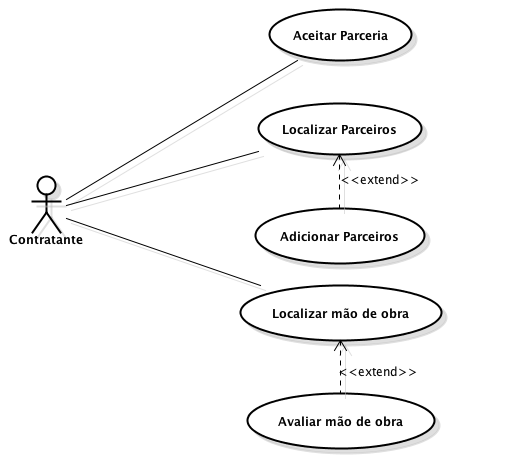
\includegraphics[scale=0.6]{./imagens/caso-de-uso.png}}
	\caption[Diagrama de caso de uso]
	{Diagrama de caso de uso. \textbf{Fonte:} Elaborado pelos autores.}
	\label{fig:exemplo1}
\end{figure}

\par Na segunda fase, análise e projeto preliminar, houve um refinamento dos requisitos levantados na fase anterior, aperfeiçoando as ações do usuário, por meio dos diagramas de casos de uso. Posterior a esta definição foram desenvolvidos os diagramas de robustez, como demonstra a Figura 17. Em paralelo, foi atualizado o modelo de domínio, acrescentando os novos atributos identificados, conforme a Figura 18. Com o modelo de domínio atualizado, foi feita a modelagem do banco de dados da aplicação, como apresenta a Figura 19.

\begin{figure}[h!]
	\centerline{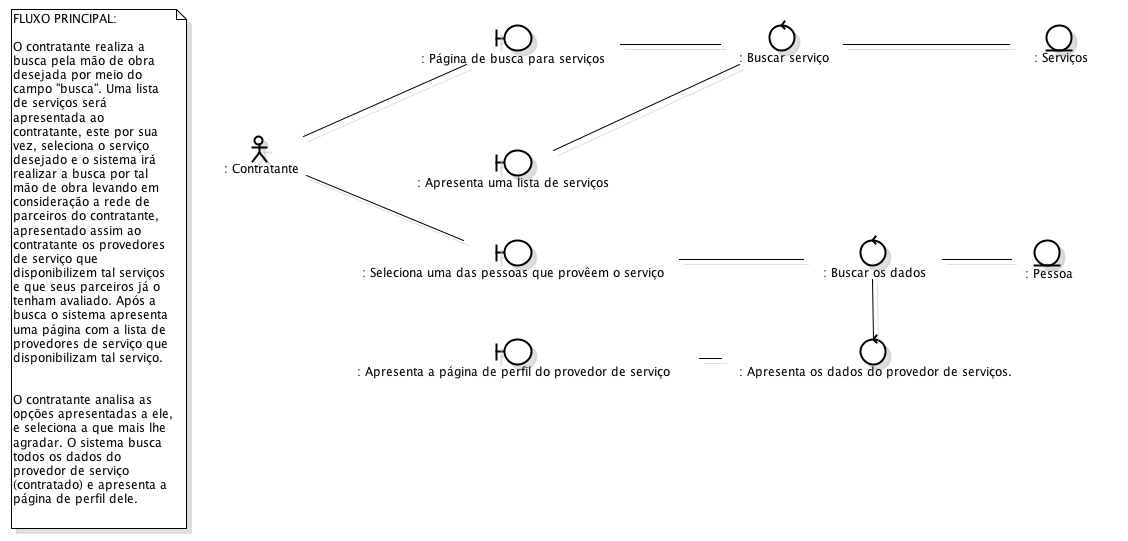
\includegraphics[scale=0.35]{./imagens/robustez.png}}
	\caption[Diagrama de robustez do caso de uso Localizar mão de obra]
	{Diagrama de robustez do caso de uso Localizar mão de obra. \textbf{Fonte:} Elaborado pelos autores.}
	\label{fig:exemplo1}
\end{figure}

\begin{figure}[h!]
	\centerline{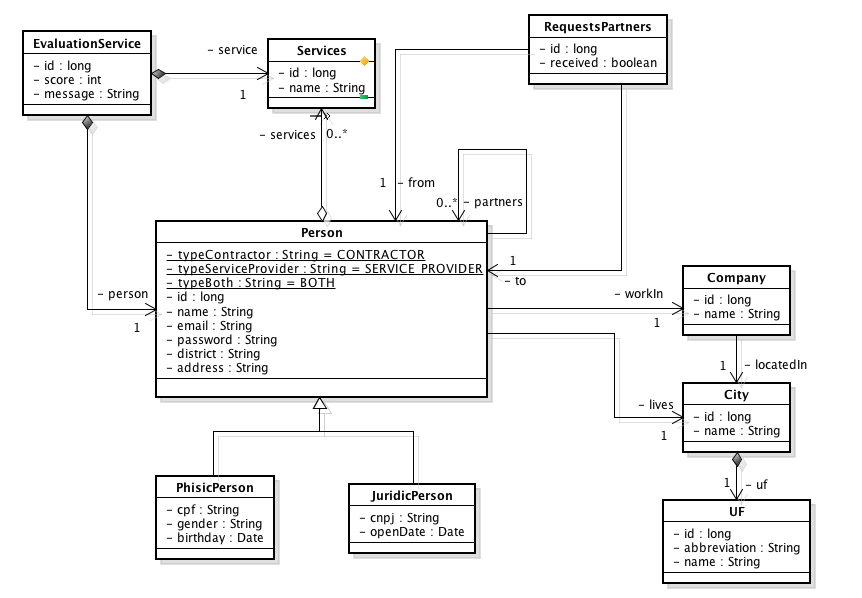
\includegraphics[scale=0.6]{./imagens/modelo-dominio-com-atributos.png}}
	\caption[Modelo de domínio atualizado]
	{Modelo de domínio atualizado. \textbf{Fonte:} Elaborado pelos autores.}
	\label{fig:exemplo1}
\end{figure} 

\begin{figure}[h!]
	\centerline{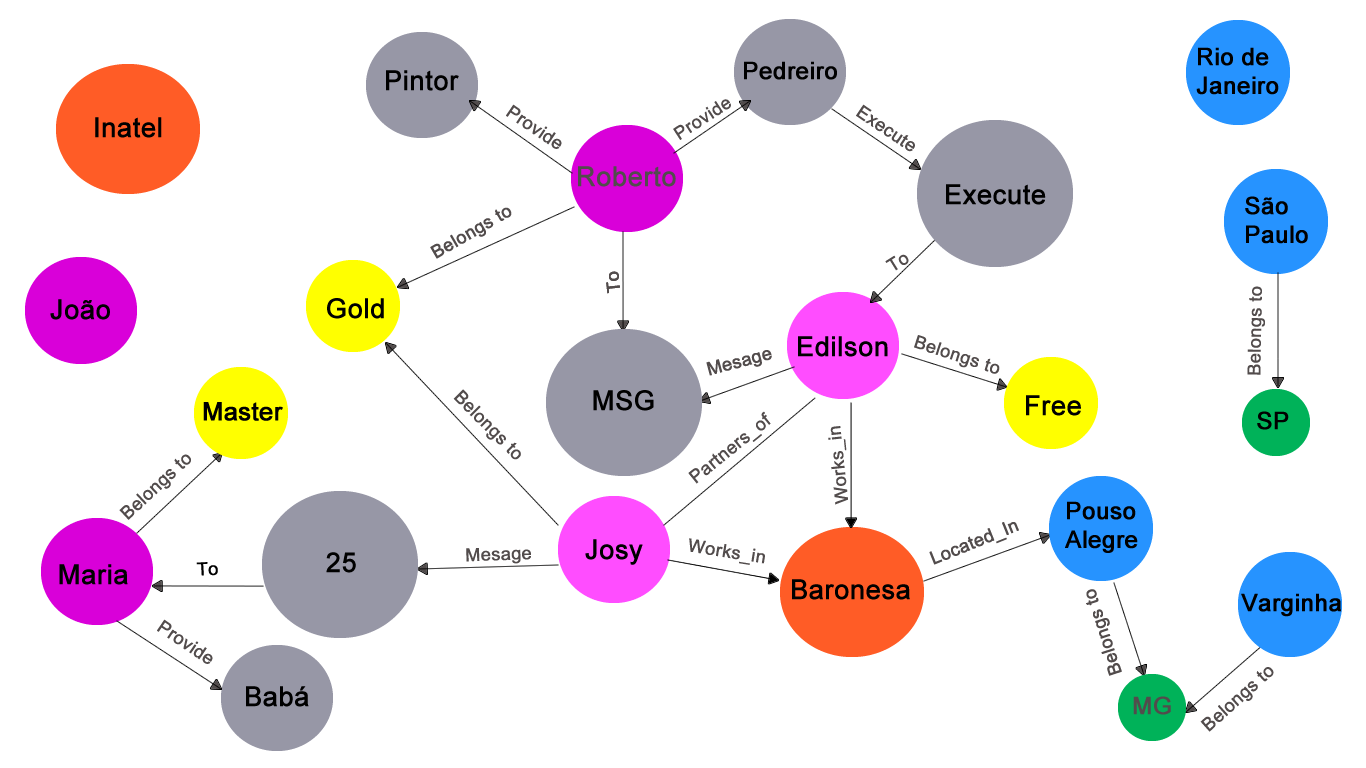
\includegraphics[scale=0.5]{./imagens/structure-all-nodes.png}}
	\caption[Modelo de dados da aplicação]
	{Modelo de dados da aplicação. \textbf{Fonte:} Elaborado pelos autores.}
	\label{fig:exemplo1}
\end{figure} 


\par Na terceira fase, definida como projeto detalhado, foram criados os diagramas de sequencia, tendo como base os casos de uso modelados na fase anterior. Esta fase tem como objetivo detalhar todo o funcionamento do \textit{software}, visando definir a melhor maneira de realizar sua implementação. A Figura 20 apresenta o diagrama de sequência do caso de uso localizar mão de obra.

\newpage
\begin{figure}[h!]
	\centerline{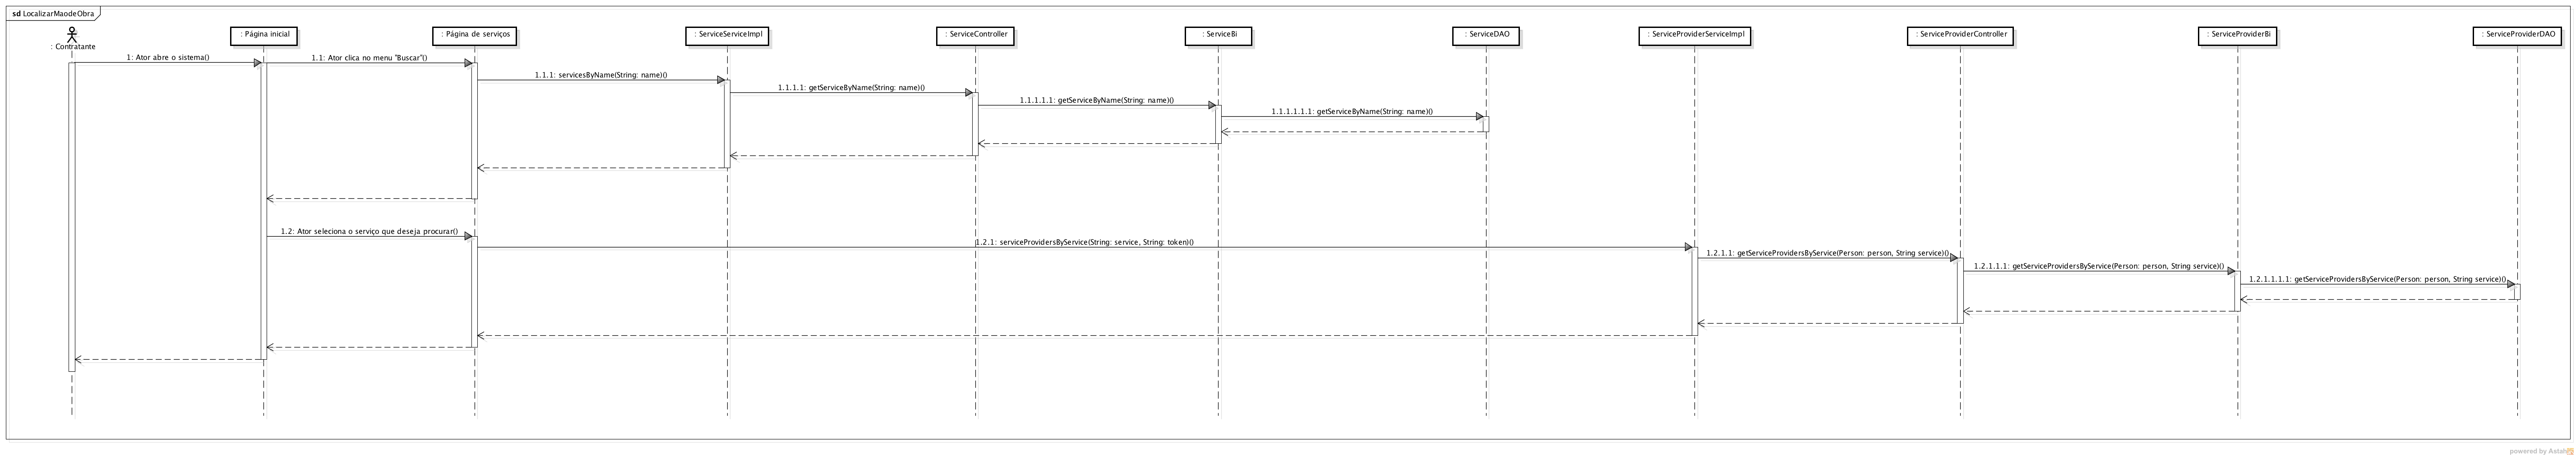
\includegraphics[angle=90,height=0.7\textheight,width=0.7\textwidth]{./imagens/sequence-localizar-mao-de-obra.png}}
	\caption[Diagrama de caso de uso]
	{Diagrama de caso de uso \textbf{Fonte:} Elaborado pelos autores.}
	\label{fig:exemplo1}
\end{figure}

\par Ainda na fase de projeto detalhado, após a modelagem dos diagramas de sequencia, as operações encontradas nestes diagramas foram adicionadas ao modelo de domínio, em conjunto com as novas classes identificadas, gerando assim, o digrama de classes como mostra a Figura 21.

\begin{figure}[h!]
	\centerline{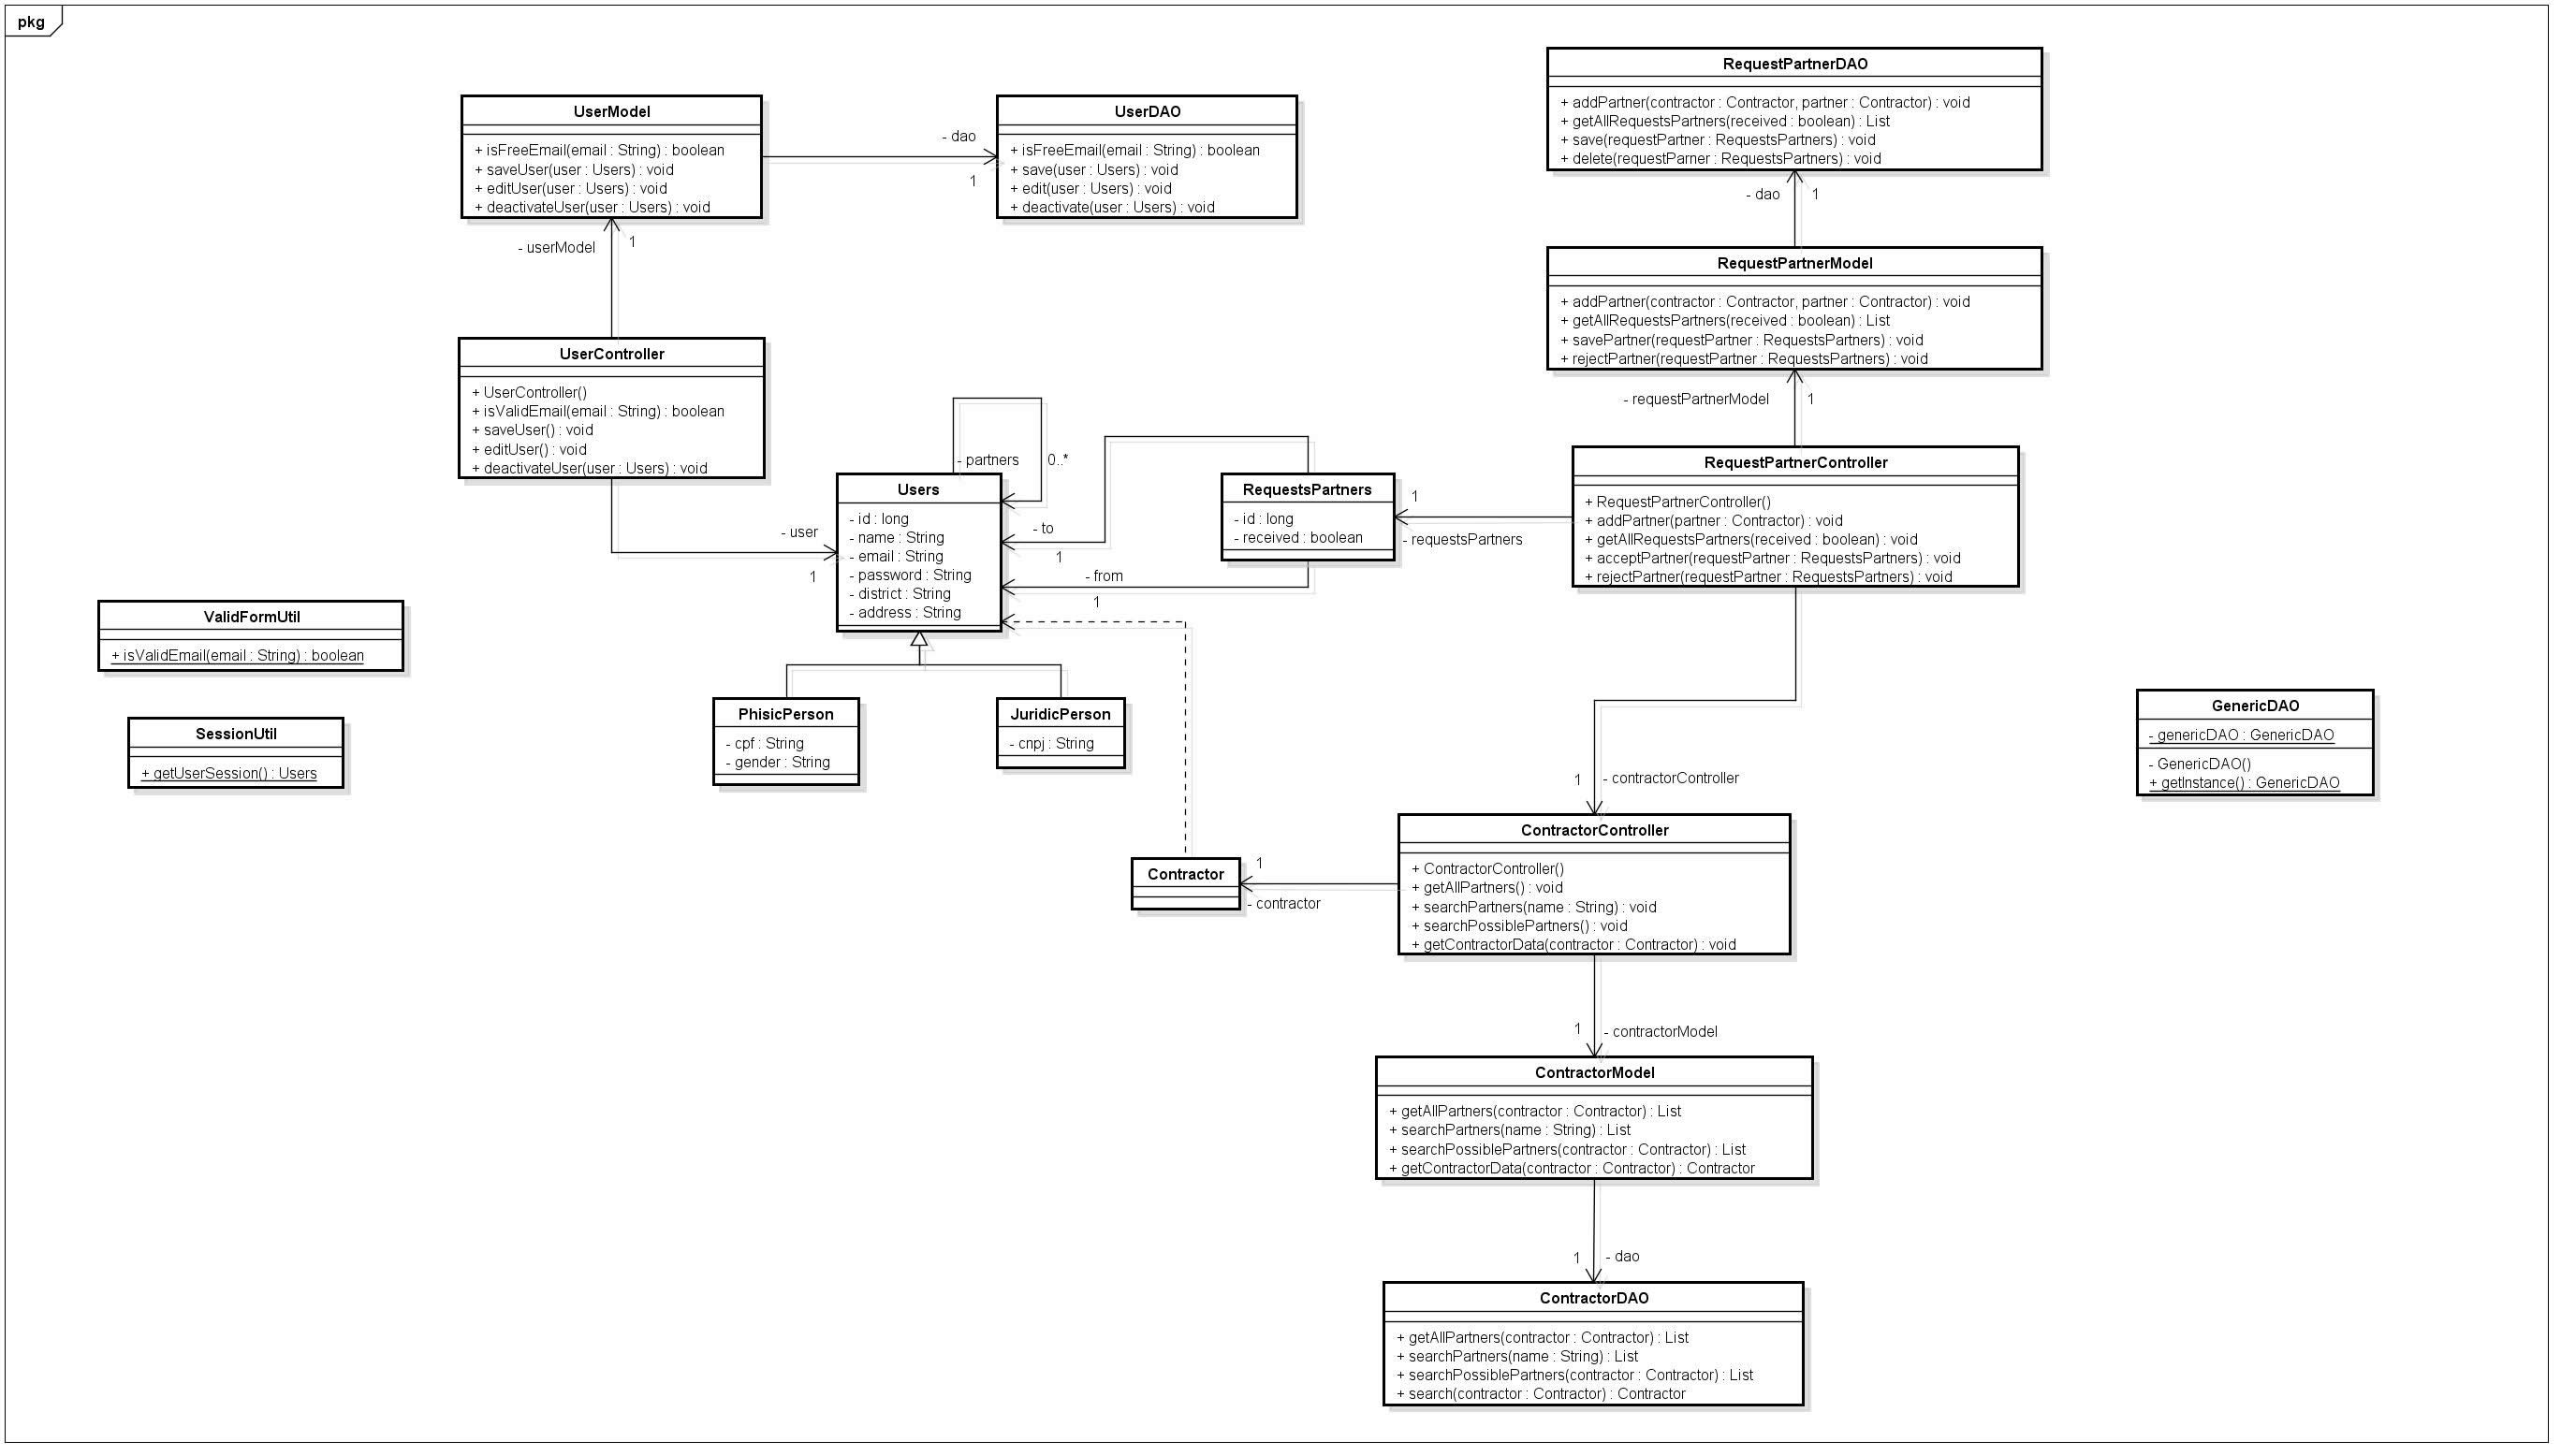
\includegraphics[angle=90,height=0.7\textheight,width=0.7\textwidth]{./imagens/classe.jpg}}
	\caption[Diagrama de classes]
	{Diagrama de classes \textbf{Fonte:} Elaborado pelos autores.}
	\label{fig:exemplo1}
\end{figure}

\newpage
\par Na quarta e última fase do ICONIX, denominada implementação, iniciou-se a preparação do ambiente, incluindo a instalação dos \textit{softwares} necessários para o desenvolvimento prático da aplicação.

\par Visto que o trabalho seria desenvolvido em equipe, foi necessário estabelecer uma ferramenta de controle de versão. Esta ferramente permitiu o gerenciamento de diferentes versões de arquivos, mantendo um histórico com as modificações que foram realizadas no decorrer do processo de desenvolvimento. Este histórico permite o retorno de alguma revisão, caso haja necessidade. A ferramenta escolhida para realizar esse controle foi o GitHub, que já havia sido utilizado em alguns trabalhos do contexto acadêmico, evitando o desprendimento de tempo para estudo de uma nova ferramenta de apoio. O GitHub é uma ferramenta bem difundida e permite que os seus usuários colaborem com os projetos que estão armazenados em seus repositórios\footnotemark[31]. A Figura 22 demonstra a tela de serviços provida pelo GitHub.

\footnotetext[31]{Repositório: local cujo desenvolvedor utiliza para armazenar os documentos relacionados ao \textit{software}.}

\begin{figure}[h!]
	\centerline{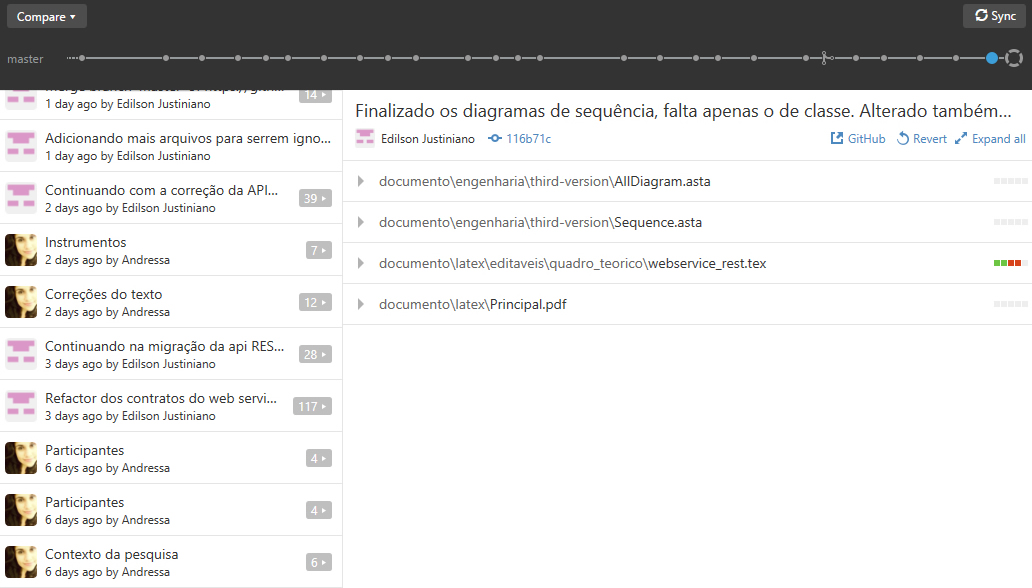
\includegraphics[scale=0.35]{./imagens/github.jpg}}
	\caption[Tela de serviços do GitHub ]
	{Tela de serviços do GitHub \textbf{Fonte:} Elaborado pelos autores.}
	\label{fig:exemplo1}
\end{figure}

\par Os passos de instalação detalhados do GitHub são descritos  no Apêndice I deste trabalho.

\par Como mencionado no quadro teórico, neste trabalho foi utilizada a linguagem Java, sendo assim necessário a utilização de uma \textit{Integrated Development Environment} - IDE\footnotemark[32] - de apoio. A IDE escolhida foi o Eclipse, pois se trata de uma ferramenta \textit{open source}, muito utilizada no mercado e que permite a escrita de um código mais legível, facilitando tarefas como \textit{debug} e configurações do trabalho.

\footnotetext[32]{IDE: \textit{Integrated Development Environment} - Aplicação contendo uma série de ferramentas para auxiliar no desenvolvimento de \textit{software}.}

\par O Eclipse possui várias ferramentas, dentre elas, pode-se citar o editor de texto, usado não somente para a escrita de códigos em Java, e também a perspectiva de configuração para servidores \textit{web}, utilizada neste trabalho, conforme apresenta a Figura 23. Por meio desta perspectiva, foi configurada a aplicação \textit{container} Tomcat na versão 7.

\newpage
\begin{figure}[h!]
	\centerline{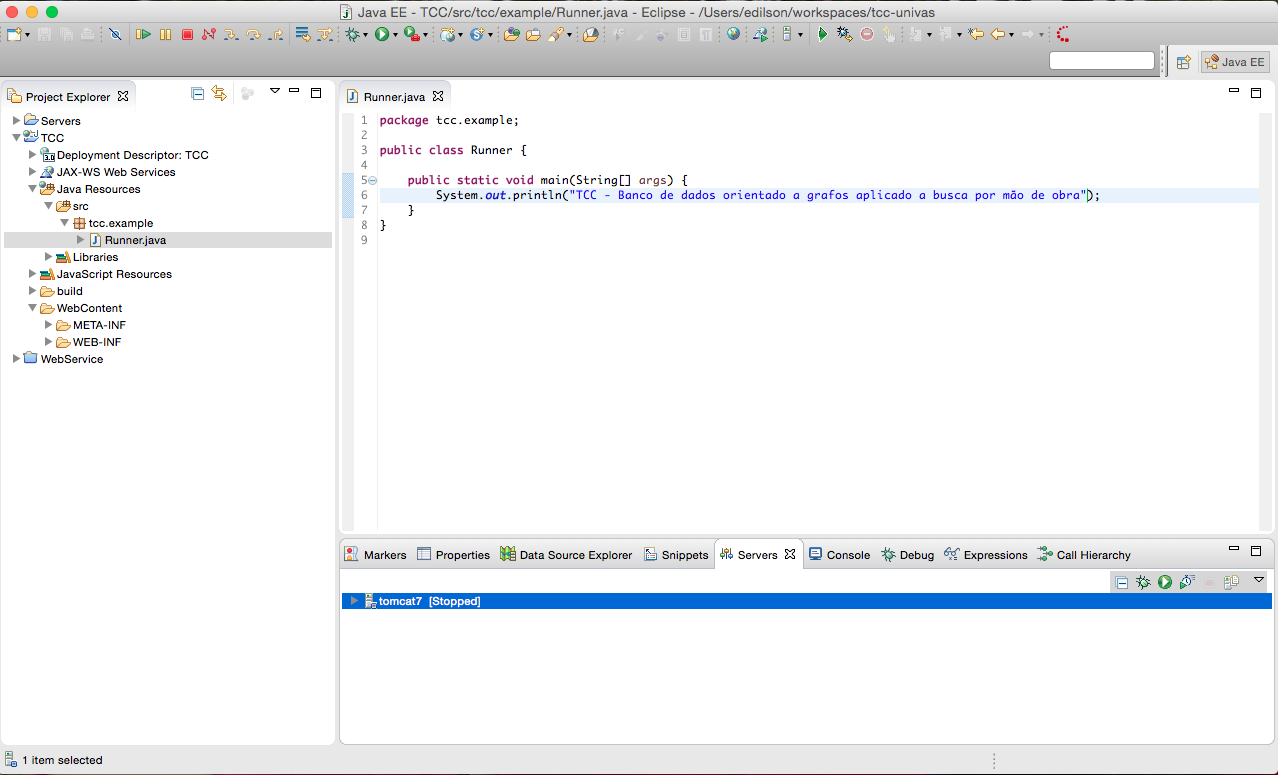
\includegraphics[scale=0.35]{./imagens/eclipse-editor-texto.png}}
	\caption[Ferramentas da IDE Eclipse]
	{Ferramentas da IDE Eclipse \textbf{Fonte:} Elaborado pelos autores.}
	\label{fig:exemplo1}
\end{figure}

\par O Tomcat desempenhou um papel fundamental na execução desta aplicação, pois serviu como hospedeiro para a aplicação Java desenvolvida neste trabalho. 

\par Os passos de instalação e configuração do Eclipse e do Tomcat são descritos no Apêndice II deste trabalho.

\par Para a escrita do código relacionado ao HTML, CSS e Javascript, foi utilizado o mesmo editor de texto citado anteriormente.

\par O trabalho fez uso de um banco de dados orientado a grafos, o Neo4j. A escolha desse banco se deu pela sua simplicidade de instalação, configuração, facilidade de integração com a API \textit{Cypher} e por disponibilizar uma API REST para acesso aos seus dados, conforme descrito no quadro teórico deste trabalho. O Neo4j faz parte do enquadramento de softwares livres, seguindo o conceito \textit{open source}, o que permite ao desenvolvedor utilizá-lo da forma que melhor lhe convier. 


\par A seguir serão detalhados os passos para a instalação do banco de dados Neo4j.

\par Para realizar o \textit{download} do instalador do banco de dados Neo4j, deve-se acessar a seguinte URL, por meio de um  navegador de internet: http://neo4j.com/download e selecionar a opção desejada. Neste trabalho como já descrito foi utilizada a versão \textit{Community}. A Figura 24 apresenta a página de \textit{download} do Neo4j.

\newpage
\begin{figure}[h!]
	\centerline{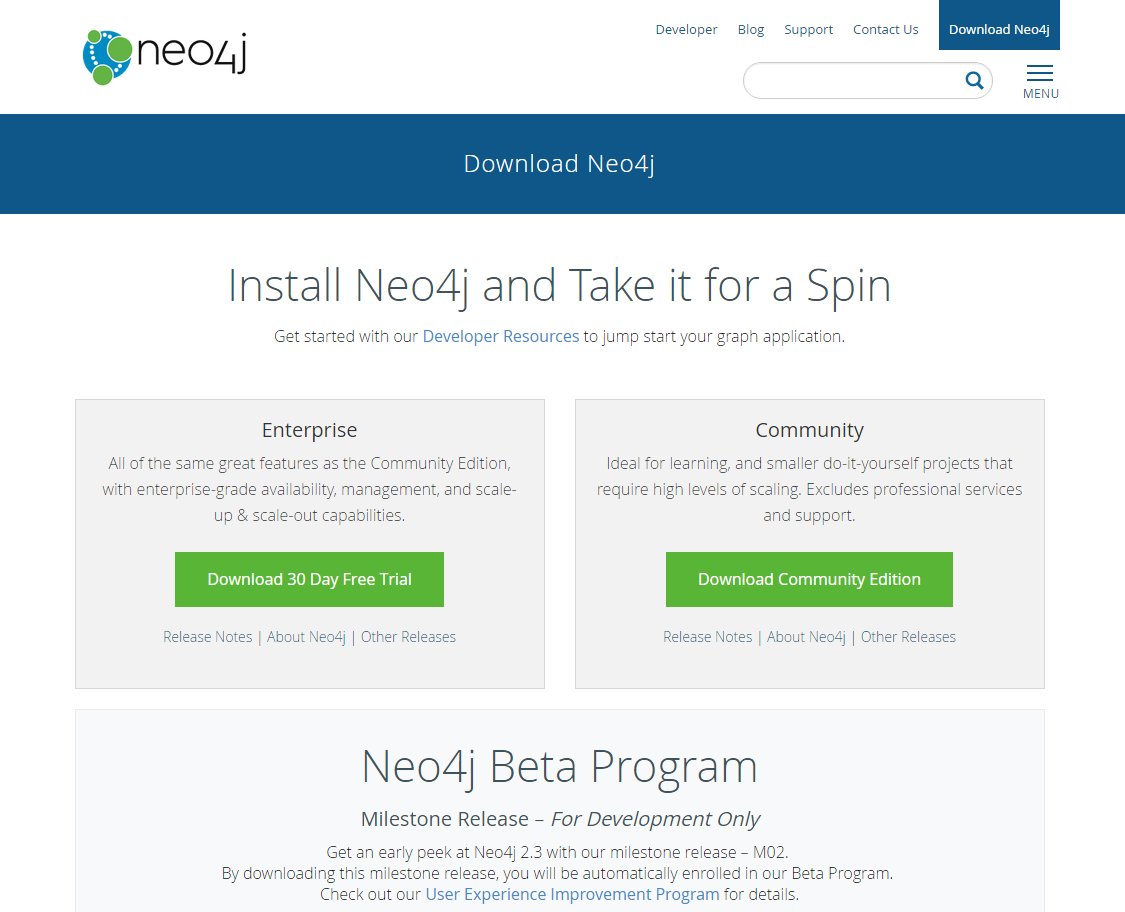
\includegraphics[scale=0.4]{./imagens/download-neo4j.png}}
	\caption[Página de download do Neo4j]
	{Página de download do Neo4j. \textbf{Fonte:} http://neo4j.com/download}
	\label{fig:exemplo1}
\end{figure}

\par Após concluído o \textit{download}, deve-se executar o arquivo. O processo de instalação se inicia e, a primeira tela apresentada ao usuário é a tela contendo uma mensagem de boas vindas, conforme demonstra a Figura 25. Nesta tela, deve-se clicar no botão \textit{Next} para prosseguir com o processo de instalação.

\begin{figure}[h!]
	\centerline{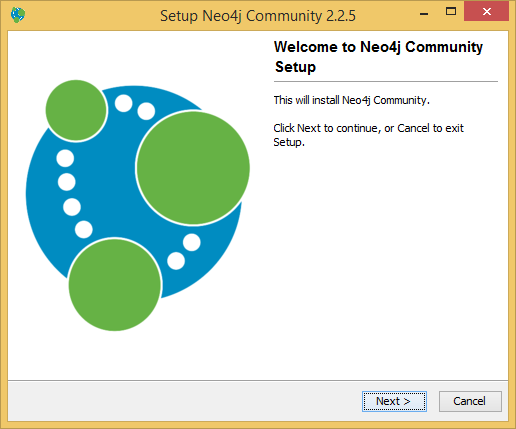
\includegraphics[scale=0.4]{./imagens/neo4j-install-step1.png}}
	\caption[Tela de boas vindas da instalação do Neo4j]
	{Tela de boas vindas da instalação do Neo4j. \textbf{Fonte:} Elaborado pelos autores.}
	\label{fig:exemplo1}
\end{figure}

\par A próxima tela apresentada ao usuário diz respeito ao contrato de uso do \textit{software}, como mostra a Figura 26. Após lê-lo, deve-se aceitar os termos do contrato e clicar em \textit{Next}.

\newpage
\begin{figure}[h!]
	\centerline{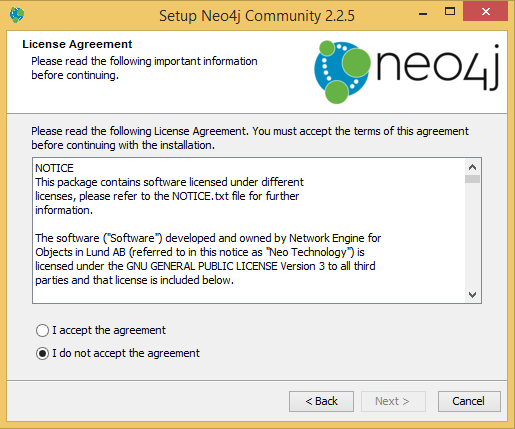
\includegraphics[scale=0.4]{./imagens/neo4j-install-step2.png}}
	\caption[Tela do contrato de uso do Neo4j]
	{Tela do contrato de uso do Neo4j. \textbf{Fonte:} Elaborado pelos autores.}
	\label{fig:exemplo1}
\end{figure}

\par Na próxima tela, conforme a Figura 27 demonstra, é definido o diretório de instalação do Neo4j. Por padrão este diretório é o mesmo das demais aplicações no \textit{Windows}, podendo ser alterado conforme a necessidade. Após definir o diretório de instalação deve-se clicar no botão \textit{Next}.

\begin{figure}[h!]
	\centerline{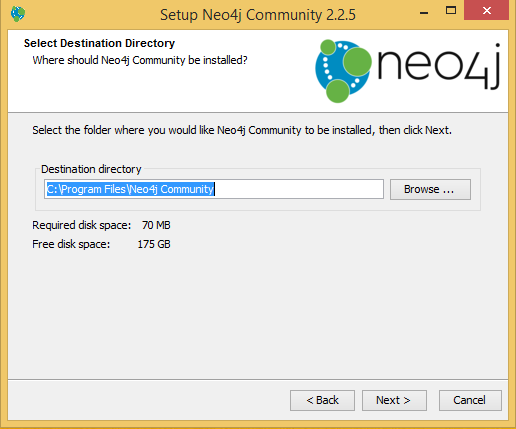
\includegraphics[scale=0.4]{./imagens/neo4j-install-step3.png}}
	\caption[Tela para definição do diretório de instalação do Neo4j]
	{Tela para definição do diretório de instalação do Neo4j. \textbf{Fonte:} Elaborado pelos autores.}
	\label{fig:exemplo1}
\end{figure}

\par Após as definições anteriores, uma tela é apresentada questionando ao usuário a respeito da criação de atalhos na área de trabalho, como é demonstrado na Figura 28. Posterior a definição dos atalhos do Neo4j, deve-se clicar no botão \textit{Next}.

\begin{figure}[h!]
	\centerline{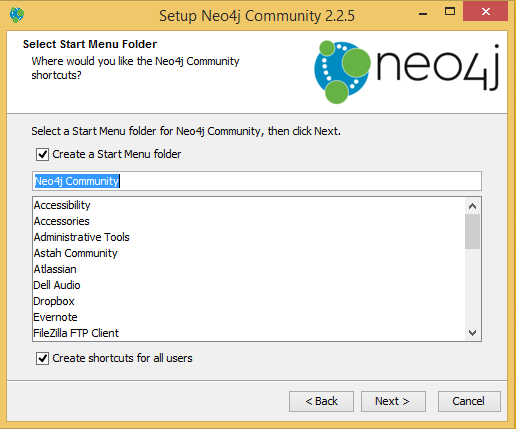
\includegraphics[scale=0.4]{./imagens/neo4j-install-step4.png}}
	\caption[Tela para criação de atalhos do Neo4j]
	{Tela para criação de atalhos do Neo4j. \textbf{Fonte:} Elaborado pelos autores.}
	\label{fig:exemplo1}
\end{figure}

\par Após realizar os procedimentos descritos para a instalação do Neo4j a tela final de instalação será apresentada, informando-o a respeito do resultado da instalação conforme demonstra a Figura 29. Clique no botão \textit{Finish} para finalizar o processo de instalação.
Após todos os passos realizados com sucesso, o Neo4j estará disponível.

\begin{figure}[h!]
	\centerline{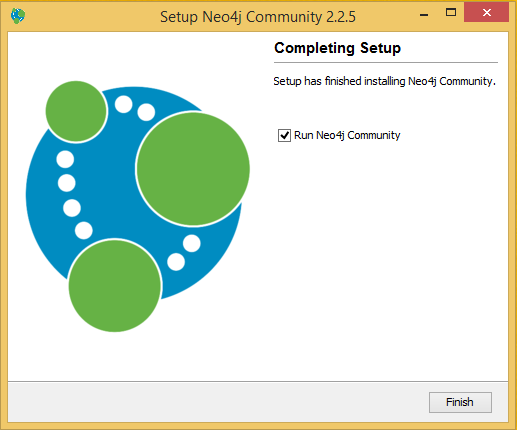
\includegraphics[scale=0.4]{./imagens/neo4j-install-step5.png}}
	\caption[Tela final de instalação do Neo4j]
	{Tela final de instalação do Neo4j. \textbf{Fonte:} Elaborado pelos autores.}
	\label{fig:exemplo1}
	
\end{figure}

\par A Figura 30 e 31 apresentam a tela inicial do banco de dados Neo4j e um exemplo de consulta realizada por meio da aplicação de gerencia da base de dados.

\begin{figure}[h!]
	\centerline{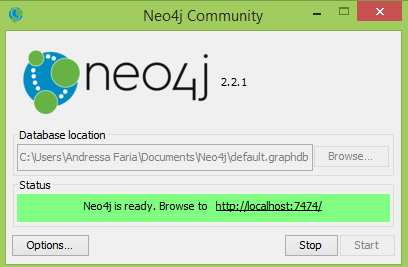
\includegraphics[scale=0.60]{./imagens/neo4j.jpg}}
	\caption[Tela de inicialização do Neo4j ]
	{Tela de inicialização do Neo4j \textbf{Fonte:} Elaborado pelos autores.}
	\label{fig:exemplo1}
\end{figure}

\begin{figure}[h!]
	\centerline{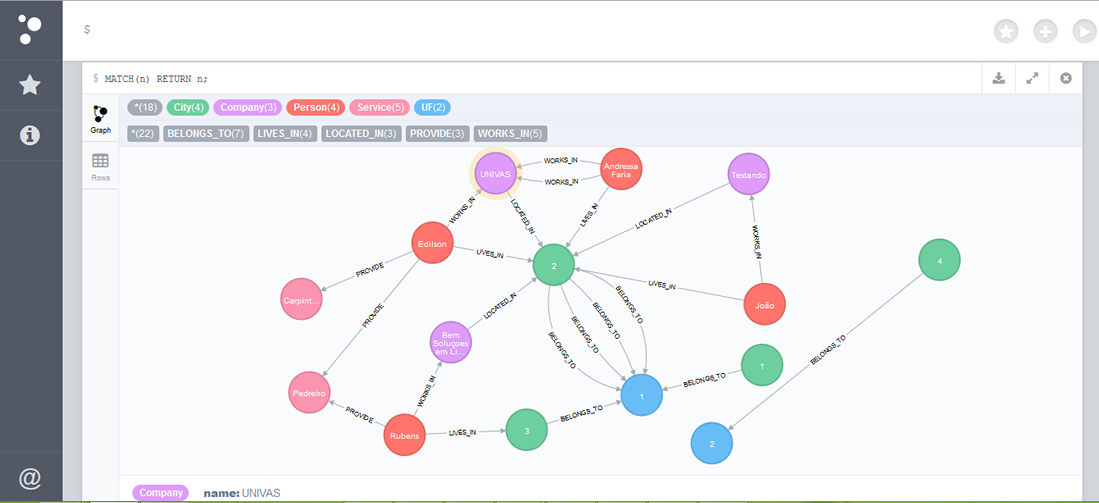
\includegraphics[scale=0.4]{./imagens/neo4j2.jpg}}
	\caption[Demonstração de uma consulta Cypher.]
	{Demonstração de uma consulta Cypher. \textbf{Fonte:} Elaborado pelos autores.}
	\label{fig:exemplo1}
\end{figure}
 
\newpage

\par Posterior a configuração do ambiente, iniciou-se o desenvolvimento propriamente dito. A princípio, utilizou-se as tecnologias Neo4j, sendo executado de forma \textit{embedded}, Primefaces e JSF. Porém não estava fluindo como o esperado, uma vez que o Neo4j utilizado desta maneira não permitia conectar ao sistema de gerenciamento da base de dados e abrir uma nova instancia de conexão simultânea, devido a limitações do próprio Neo4j, uma vez que um processo Java já ocupava tal conexão com o \textit{socket} do banco de dados.

\par Outro problema encontrado ao utilizar tais tecnologias foi que tanto a parte cliente (\textit{front end}) quanto a parte servidor (\textit{back end}) se encontravam totalmente acoplados em uma aplicação Java \textit{web}, portanto, a cada alteração realizada havia a necessidade de recompilar, construir e publicar a aplicação no servidor \textit{web}, impedindo a agilidade no desenvolvimento do \textit{software}. Por esses motivos decidiu-se mudar algumas das tecnologias utilizadas no \textit{front end} e a maneira como o banco de dados era acessado até então. 

\par Posterior a esse incidente, passou-se a utilizar então as linguagens HTML 5, CSS 3, Javascript e o \textit{framework} Angular JS para auxiliar no desenvolvimento do \textit{front end}, ao invés de Primefaces e JSF. Para acesso ao banco de dados, lançou-se mão da forma \textit{embedded} e passou-se a utilizar a API REST disponibilizada pelo próprio banco. Tais decisões nos permitiram desacoplar o sistema e manter o \textit{front end} e o \textit{back end} independentes, evitando assim, que o mesmo problema voltasse a ocorrer.

\par Como a forma de conexão ao banco de dados foi alterada, houve-se a necessidade de reescrever a classe responsável por realizar esta conexão. Ao utilizar esta nova abordagem de conexão ao banco de dados, foi necessário informar o \textit{hostname} e a porta IP cujo banco está instalado e o diretório onde os dados estão localizados internamente no Neo4j. Neste trabalho foi utilizado o diretório padrão (/db/data). Após realizada esta configuração, foi necessário acrescentar o parâmetro ''/cypher'' à criação da instância de conexão, a fim de utilizar a API \textit{Cypher} em conjunto com esta nova abordagem, conforme apresenta a Figura 32.

\begin{figure}[h!]
	\centerline{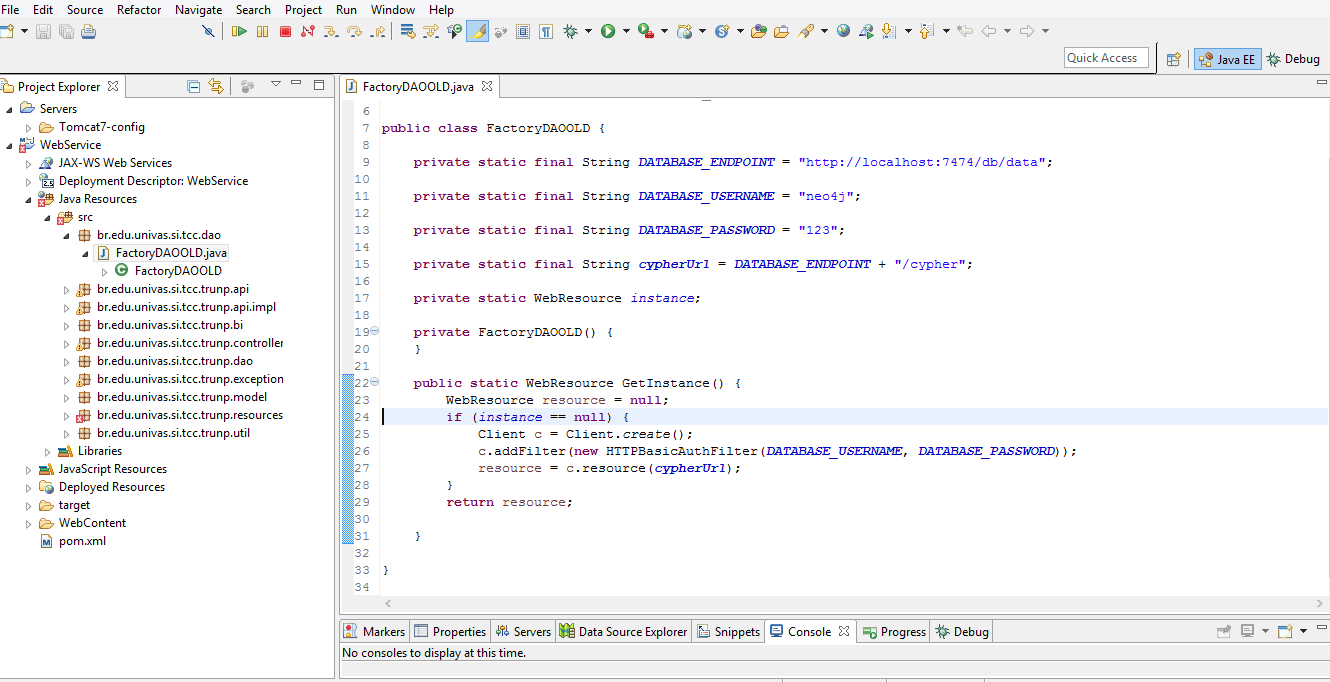
\includegraphics[scale=0.35]{./imagens/conexao-banco.jpg}}
	\caption[Código de comunicação com o banco]
	{Código de comunicação com o banco \textbf{Fonte:} Elaborado pelos autores.}
	\label{fig:exemplo1}
\end{figure}

\par Após realizar a mudança de tecnologias, foram executados alguns testes para compreender o funcionamento do \textit{web service} REST e em paralelo, foi feito o levantamento dos materiais de referência do \textit{framework} Angular JS. Foi preciso realizar testes para validar a conexão com o banco de dados Neo4j via API REST, fornecida por ele. Também foram realizados testes para envio de requisições e recebimento de respostas do \textit{web service} REST, utilizando o Angular JS. Para validar a conexão ao banco de dados via API REST foi necessário desenvolver algumas consultas em \textit{cypher} como apresenta a Figura 33.

\newpage 
\begin{figure}[h!]
	\centerline{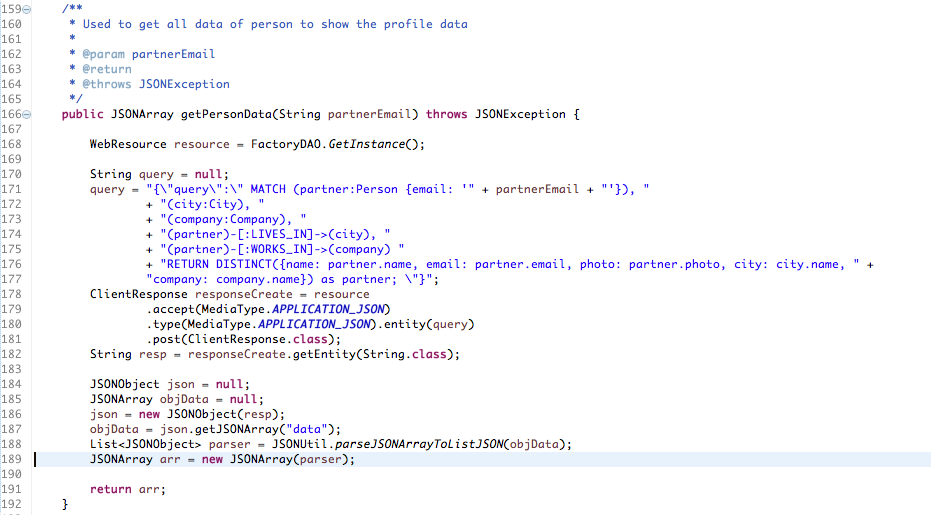
\includegraphics[scale=0.45]{./imagens/query-cypher.png}}
	\caption[Exemplo de consulta usando a API \textit{cypher}]
	{Exemplo de consulta usando a API \textit{cypher}. \textbf{Fonte:} Elaborado pelos autores.}
	\label{fig:exemplo1}
\end{figure}

\par Ao realizar estes testes foi constatado que seria necessário desenvolver uma maneira de converter os resultados das buscas realizadas no banco de dados Neo4j que, por padrão não retorna os resultados no formato JSON comum, portanto, houve-se a preocupação em tratar estas respostas, a fim de retornar um JSON válido ao usuário que futuramente viria a utilizar a API REST fornecida por este \textit{software}. É possível visualizar este tratamento na Figura 33. 
 
\par A partir deste ponto, a aplicação estava totalmente desacoplada, sendo necessário realizar uma configuração, a fim de permitir que as requisições enviadas pelo \textit{front end} fossem aceitas pelo \textit{back end}, localizado em outro domínio.

\par Devido a mudança de tecnologias já comentadas, houve-se a necessidade de atualizar os diagramas de sequência e de classe, inserindo os contratos de serviços do \textit{web service} REST. Com a definição deste contrato, deu-se início ao desenvolvimento dos casos de uso, identificados na primeira fase do ICONIX. 

\par Posterior a realização dos testes e da escolha definitiva da arquitetura que seria utilizada, iniciou-se a implementação dos casos de uso. O primeiro a ser implementado foi o caso de uso de criação de conta. Para este caso de uso, teve-se o cuidado de criar um mecanismo de criptografia de dados sigilosos, como usuário e senha, visando garantir a segurança da aplicação. Estas informações criptografadas são enviadas a cada requisição e validadas pelo \textit{web service}, sendo atualizadas caso sejam válidas, tornado mais complexo a quebra desta criptografia. Este mecanismo foi desenvolvido com base no sistema de \textit{login} via \textit{token}. Segundo o embasamento usado na criação de contas, deu-se início ao desenvolvimento do sistema de \textit{login} e \textit{logoff}, que também utilizam o conceito de criptografia via \textit{token}. A Figura 34 apresenta a página de \textit{login}.

\begin{figure}[h!]
	\centerline{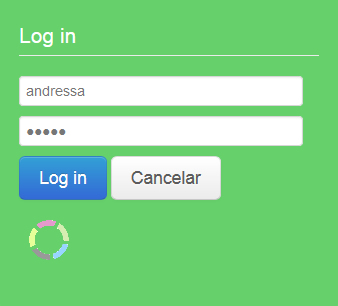
\includegraphics[scale=0.60]{./imagens/login.jpg}}
	\caption[Tela de login ]
	{Tela de login \textbf{Fonte:} Elaborado pelos autores.}
	\label{fig:exemplo1}
\end{figure}

\par Com o funcionamento do sistema de \textit{login}, passou-se a desenvolver à página inicial da aplicação, contendo as informações que são restritas ao usuário cadastrado. O sistema apresenta uma página inicial diferente para cada tipo de conta, sendo elas: contratantes, provedores de serviço ou ambos, contendo apenas as informações que são liberadas de acordo com o acesso do usuário, sendo essas informações relatórios, últimas atualizações na rede de parceiros, avaliações de serviços e prováveis parceiros. A página inicial do tipo contratante é apresentada na Figura 35.

\begin{figure}[h!]
	\centerline{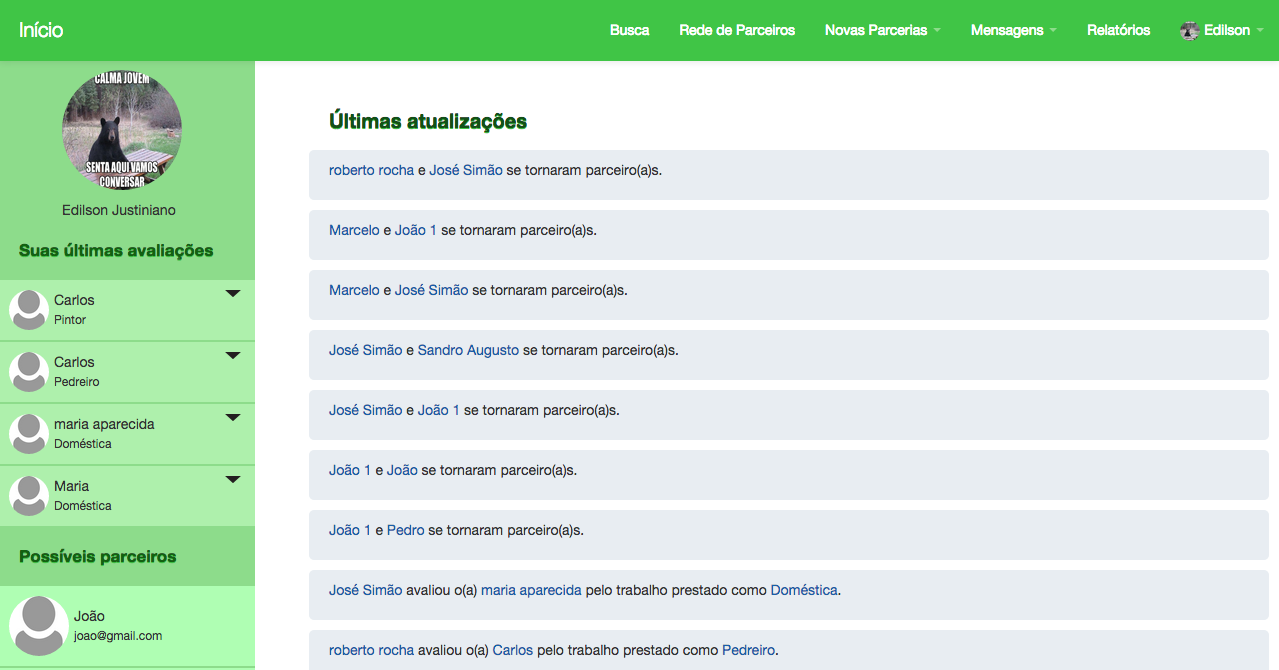
\includegraphics[scale=0.35]{./imagens/home-contratante.png}}
	\caption[Página inicial do usuário contratante]
	{Página inicial do usuário contratante \textbf{Fonte:} Elaborado pelos autores.}
	\label{fig:exemplo1}
\end{figure}


\par O caso de uso localizar parceiros foi desenvolvido após a conclusão do caso de uso criar conta. A lógica deste caso de uso consiste em buscar por possíveis parceiros, com base na rede de parceria do contrante. A Figura 36 apresenta esta busca.

\begin{figure}[h!]
	\centerline{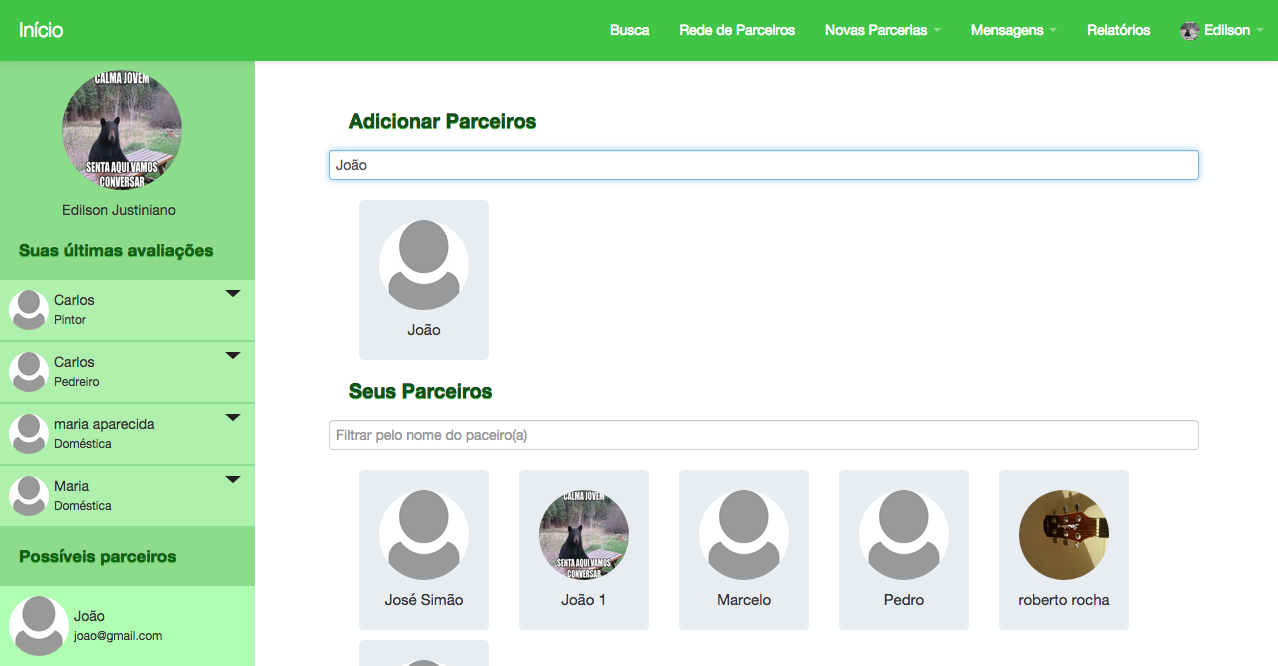
\includegraphics[scale=0.35]{./imagens/localizar-parceiro.png}}
	\caption[Página de localização de parceiros]
	{Página de localização de parceiros \textbf{Fonte:} Elaborado pelos autores.}
	\label{fig:exemplo1}
\end{figure}

\newpage



\par Ainda relacionado ao tipo de conta contratante ou ambos, foi implementado o caso de uso adicionar parceiro, que permite ao usuário convidar um possível parceiro para fazer parte da sua rede. Após a implementação da lógica para adicionar um novo parceiro, houve-se a necessidade de implementar o serviço de requisições de parcerias, uma vez que não bastava apenas um contratante convidar outro para se tornarem parceiros, mas sim que o contratante convidado aceitasse sua solicitação de parceria, para assim se tornarem parceiros. Visando disponibilizar estas solicitações de forma agradável ao usuário, foi desenvolvida uma funcionalidade para que o usuário pudesse aceitar ou rejeitar a solicitação enviada à ele.

\par Após realizada a implementação do caso de uso adicionar parceiro, houve-se a necessidade de desenvolver a busca por todos os usuários que possuíam o tipo de conta contratante ou ambos e que possuíam um relacionamento de parceria com o usuário autenticado no sistema, além da funcionalidade de localizar novos parceiros, baseando-se na localização da empresa na qual o usuário trabalha e na cidade onde ele vive, sempre ordenando os resultados por meio da quantidade de parceiros em comum. 

\par O caso de uso gerenciar serviços foi implementado em sequência, abrangendo as principais funcionalidades de gerenciamento: cadastrar e adicionar um novo serviço ao usuário, cujo tipo de conta é provedor de serviços, listar os serviços atribuídos a ele, e remover serviços quando necessário. Visando melhorar a usabilidade, foi implementado um mecanismo de busca, que permitiu filtrar os resultados por meio de um campo que possui a função  auto completar, evitando assim, possíveis erros e diminuindo o tempo gasto pelo usuário para adicionar o serviço. A função realiza a busca em uma lista de serviços anteriormente cadastrados, no entanto, caso não haja o serviço solicitado, o usuário tem a liberdade de cadastrá-lo e atribuí-lo a si mesmo.

\par A partir deste ponto, foi possível iniciar o desenvolvimento do caso de uso localizar mão de obra, uma vez que, este caso de uso dependia diretamente das implementações das funcionalidades adicionar parceiros para os usuários contratantes e adicionar serviços aos provedores de serviço. Para facilitar a localização e deixar o \textit{software} mais usual, esta busca se baseia inicialmente no serviço buscado pelo usuário, sendo posteriormente modificada para também levar em consideração a funcionalidade avaliar serviço que foi implementada paralelamente. A avaliação de serviço permite ao contratante dar uma nota ao serviço que foi prestado a ele. Com estas informações foi possível desenvolver uma busca que levaria em consideração, além destas informações, a rede de parceiros do usuário contratante, a fim de lhe apresentar as melhores opções possíveis.

\par A fim de abranger a busca e possibilitar que novos prestadores de serviços sejam avaliados pelos contratantes, a consulta que antes apresentava apenas provedores de serviços que possuíam avaliações, sendo elas, positivas ou negativas, foi ampliada, possibilitando que profissionais não avaliados também entrassem na lista de prováveis provedores de serviços.

\par Para auxiliar na tomada de decisão do usuário contratante, foi implementada uma funcionalidade que realiza o cálculo da média de avaliações de um serviço prestado por um profissional temporário, tendo como base as avaliações já realizadas pela rede de parceiros do usuário autenticado, da empresa onde ele trabalha e da cidade onde vive, oferecendo assim uma forma simples de obter acesso a qualidade do serviço prestado.

\par Após realizada todas as implementações já descritas, houve-se a preocupação de desenvolver uma interface, que além de amigável fosse prática ao usuário, desta forma, foi disponibilizada algumas informações relevantes, que auxiliam o usuário a compreender o que está ocorrendo em sua rede de parceria. Como exemplo é possível citar a lista de parceiros em comum entre o usuário autenticado no sistema e um determinado contratante por meio da página de perfil dele.

\par A fim de agregar mais funcionalidades para o usuário provedor de serviços, foi criado na página inicial do \textit{software} uma funcionalidade que visa apresentar algumas dicas interessantes que contribui com a sua imagem perante ao \textit{software}, levando-o assim a obter uma quantidade maior de oportunidades de trabalho.

\par Para finalizar o desenvolvimento será necessário desenvolver alguns gráficos que apresentem ao usuário informações a respeito da qualidade do serviço prestado pelo provedor de serviços, comparando-os com os demais prestadores, porém estes gráficos ainda não foram implementados até o momento.
